\documentclass{article}
\usepackage[utf8]{inputenc}
\usepackage{graphicx}
\usepackage{subfig}
\usepackage{xcolor}
\usepackage{amsmath}
\usepackage{nccmath}
\usepackage{booktabs}
\usepackage{multirow}
\usepackage[margin=1in]{geometry}

\begin{document}
	\begin{center}
    
		\LARGE{\textbf{Automatic Path Planning for Agricultural Irrigation Vehicles}} \\
        \vspace{1em}
        \normalsize\textbf{Yunfeng Xin, Zhengyu Chen, Feng Chen} \\
        \vspace{1em}
        \large{Progress Report} \\
        \vspace{1em}
     
	\end{center}
    \begin{normalsize}
    
    	\section{Introduction:}
        
            Coverage Path Planning(CPP) is a well-studied topic in recent years. Different approaches is applied to solve this type of problem including A* search\cite{b1}, dynamic programming\cite{b2} and neutral network\cite{b3}. Luis Piardi\cite{b4} suggested using Q-learning to optimize CPP, however, the result turned to involve unnecessary turns in the path planning. An increasing number of turns is inefficient for agricultural vehicles since it introduced more acceleration and deceleration in the real-world application. In this project, we plan to solve the problem by using reinforcement learning. The goal for this project is to find an optimal complete coverage path with a relatively fewer number of turns. 
      
		\section{Model:}
		    \subsection{Model Description:}
		    
		        To simplify our problem, the graph will be discrete and contains connected blocks. The graph has a starting block indicating the initial position of the agent and positions of the obstacles which the agent needs to avoid. The agent will try to traverse the graph with the least travelling distance. The agent is only allowed to move up, down, left, and right. Additionally, we want to impose real-world constraints such as requiring the least number of turns because it is costly for agricultural vehicles to make a turn. Finally, the agent will output an episode of actions indicating a path from the start to the end point.
		        
		    \subsection{Map:}
		        
		        Since we will be representing our target area with a $M \times N$ grid, the data section of the map is simply implemented as a numpy 2d-array, where we use different values to represent different status of each grid block. The available status are \{BLOCKED, UNVISITED, VISITED\}. To simplify the coding effort for various agents, the map class contains various helper functions to check the status of a block (e.g. if the visited index is out of bound, it will simply return a status of BLOCKED). 
		        
		    \subsection{State Encoding:}
    	        
    	        A simple way of encoding the state will be combining the current map information, and the current location of the agent. However, such a naive way of encoding the states causes an issue: since there are multiple way of completing the current traversal of the map, the agent will have no way of learning how well it is performing (e.g. the number of turns). In the figure below shows two identical map states with very different performance implications in terms of the number of turns (and thus the amount of fuel used). Furthermore, different agents might need different state information, and it will be painful to implement all these different state transitions. Thus, our team implemented a unified bookkeeping wrapper for recording all the necessary state variables (number of turns, current episode, map information, etc.) and can be retrieved on demand, which will be discussed in detail in the next section.
    	        
    	        \begin{figure}[htp]
                    \centering
                    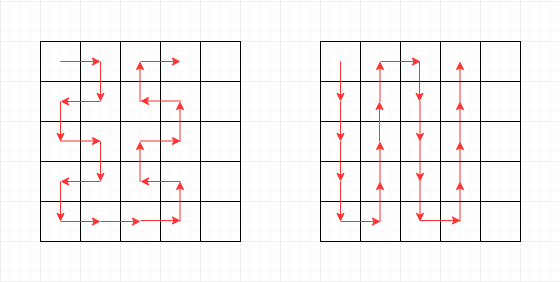
\includegraphics[width=10cm]{state.png}
                    \caption{Example of two traversal paths that has the same visited blocks in the map data and the same current agent location, but with different performance implications in terms of the number of turns.}
                \end{figure}
		        
    	    \subsection{Bookkeeping State Wrapper:}
    	        
    	        The bookkeeping wrapper serves as an unified interface environment for the agents to interact with. It provides options to set the content of the map, as well as other necessary state information such as the starting point for the agent, during the initialization of the wrapper class object. Users can simply pass in the desired map size and a list of obstacles in the map and the bookkeeping wrapper will generate the resulting map automatically.\par
    	        The bookkeeper also provides many useful utility functions such as providing the number of remaining nodes to be visited, returning a list of available successor actions (so that the agent don't bump into obstacles), and even extracting a portion of the map around the agent.\par
    	        During simulation, the agent interacts with the environment by inquiring the available successor actions, and decides on which action to take. Subsequently the agent calls the step() function to take the action, and the environment will make all the necessary state transitions and keep the information of the next state. The agent can then query the environment for all the state variables it needs to assemble its own next state encoding.
    	        
    	    
		    \subsection{Statistics and Visualization:}
    	        
    	        As we will use different evaluation metrics to assess different agents, the wrapper class also keeps counting the number of turns a agent has performed, and the total distance the agent has travelled. Based on these statistics, we can implement different scoring models and compare the performance of different agents under different criteria. \par
    	        In order to make the state information more intuitive to human users, the environment also provides a basic visualization option, which visualizes the landscape of the current map, the location of the agent, and various obstacles.
		    
            
        \section{Algorithm:}
            
            \subsection{Baseline:}
            
                The baseline algorithm is A*, following the problem set up described in the Section 2. The strategy for A* is:
                \begin{enumerate}
                    \item If previous action is available in current state, assign previous action so that the number of turns can be reduced.
                    \item If previous action is not available, greedy assign new actions which lead agent to unvisited grid
                    \item If all neighbor grids are visited, greedy choose the unvisited grid and use A* to generate a path to the unvisited grid.
                    
                    \end{enumerate}
            
            \subsection{Brute Force:}
            
                The brute force algorithm is to try 'all' possible solutions and find the best one. The 'all' here is actually ill-defined, as for a simple $2\times2$ map there exists infinite solutions. We can always go back and forth for any times before finishing (this is because we don't prohibit revisit the same site). So we should set a limit for the call stack anyway. In the brute force algorithm, we should set the limit much bigger than the number of grids. Denote the limit of call stack as $D$. The complexity is on the order of $O(4^D)$. This becomes impractical for a real large scale map. However, brute force algorithm will always give the optimal solution. Here, we use the breadth first search (BFS) as our brute force algorithm. The algorithm can only run for a such small map as $3\times3$ in a reasonable time.
                
            \subsection{Depth Limited Search:}
            
                In order to tackle the exponentially exploded complexity in the brute force algorithm, we develop a compromised algorithm. The general idea is to set a much smaller depth limit for the previous BFS. After the search reaches maximum depth, we introduce an evaluation function to return an estimated rewards based on the current path and the entire map. The algorithm will choose the action with maximum expected rewards. Equation (1) shows the key part of the algorithm, where $V(s,d)$ is expected rewards, Utility$(s)$ is the final evaluation function and actions denotes the set of current available actions regarding the state $s$. Isend$(s)$ is true when we traverse the entire map. This is actually a recursive function, and our algorithm will be similar to BFS except that we limit the call stack depth to $d$. The complexity will be on the order of $O(4^dMN)$. Again $M$ and $N$ are the dimensions of the map. However, this algorithm doesn't promise to find the optimal solution. In some cases, the agent may be trapped and the algorithm cannot give the solution.
                
            \begin{ceqn}
            \begin{align}
                V(s,d)=\left\{
                \begin{array}{ll}
                                      Utility(s) & \text{Isend(s)}\\
                                      Evaluation(s) & \text{d=0}\\
                                      \max_{a \in actions} V(succeed(s,a),d-1) & \text{Otherwise}\\
                                    \end{array}
                \right.
            \end{align}
            \end{ceqn}

            
            \subsection{Local-approximation Bounded Search:}
            
                Here, we develop another algorithm to tackle the exponentially exploded complexity in the brute force algorithm. The idea is that instead of using all the map we use the local map and implement the brute force algorithm to give the actions. The local map is much smaller than the real map. Denoting the dimension of the local map as $L$, the complexity is on the order of $O(4^{L^2}MN)$. In each step, we first obtain the local map, and run BFS on it to obtain the action. Repeat until the entire map is traversed. Again, this algorithm doesn't promise optimal solution. And because we only consider the local properties, the agent may be trapped in complicated map. In such case, the algorithm will enter infinite loop and even cannot find the solution.
            
            
        \section{Preliminary Results:}
        In this section, we generate analyze the algorithm performance in 3 cases:no obstacle, one obstacle and two obstacle. 
        
        The result indicate that all of the algorithms are able to generate a fully coverage path for no obstacle and one obstacle case. 
        
        Local-approximation search approach trapped in the two obstacle case. 
        
        In Figure.\ref{fig:algovsA*}, Green line means basic path, yellow line means revisited path, and line means trapped path. Based on Table \ref{comparison table} we can conclude that in the small and naive case(i.e., 5$\times$ 5 grid, on or only one obstacle) A* and Local-approximation Search provides almost same quality of solutions. 
        Future work can be test and compare these algorithm in difference cases and try to explore better algorithm. 
        \begin{figure}
    \centering
    \begin{minipage}{.33\textwidth}
      \centering
      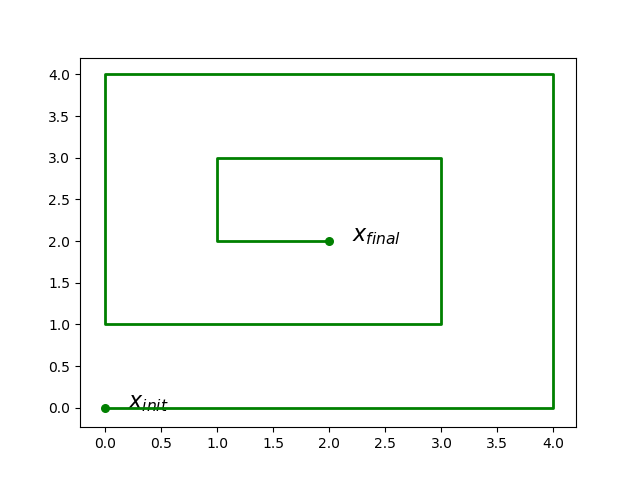
\includegraphics[width=\linewidth]{deliverables/Astar_output_no_obs.png}
      \caption{A* no obstacle case}
    \end{minipage}%
    \begin{minipage}{.33\textwidth}
      \centering
      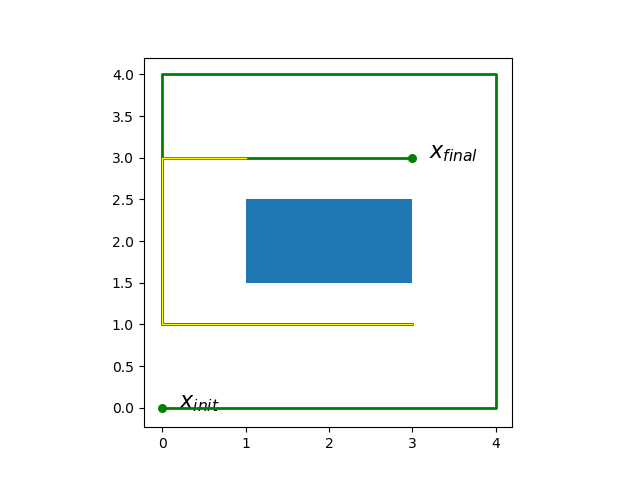
\includegraphics[width=\linewidth]{deliverables/Astar_output_1_obs.png} 
      \caption{A* 1 obstacle case}
    \end{minipage}%
    \begin{minipage}{.33\textwidth}
      \centering
      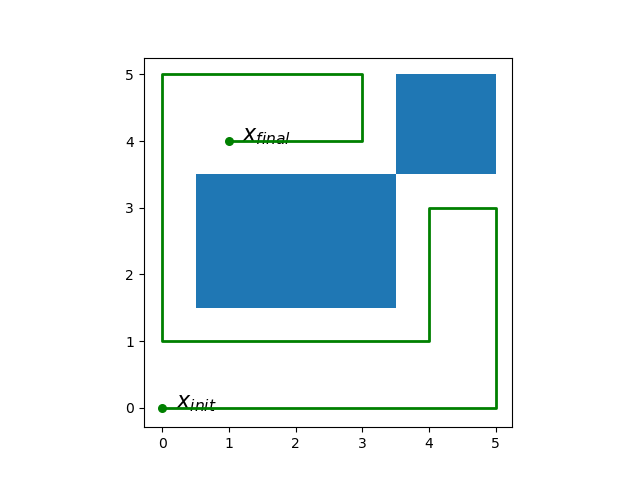
\includegraphics[width=\linewidth]{deliverables/Astar_output_2_obs.png}% placeholder
      \caption{A* 2 obstacles case}
    \end{minipage}
    \begin{minipage}{.33\textwidth}
      \centering
      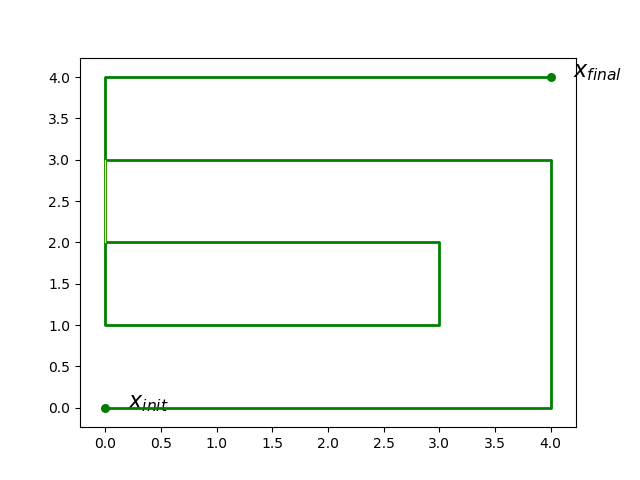
\includegraphics[width=\linewidth]{deliverables/DLS_no_obs.png}
      \caption{depth-limited Search no obstacle case }
    \end{minipage}%
    \begin{minipage}{.33\textwidth}
      \centering
      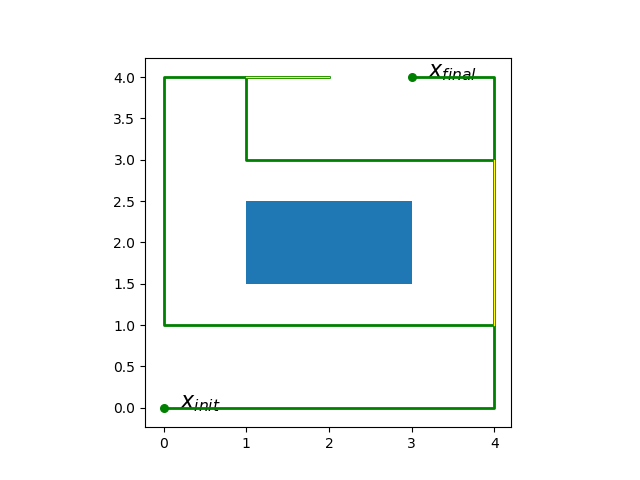
\includegraphics[width=\linewidth]{deliverables/DLS_1_obs.png}
      \caption{depth-limited Search 1 obstacle case }
    \end{minipage}%
        \begin{minipage}{.33\textwidth}
      \centering
      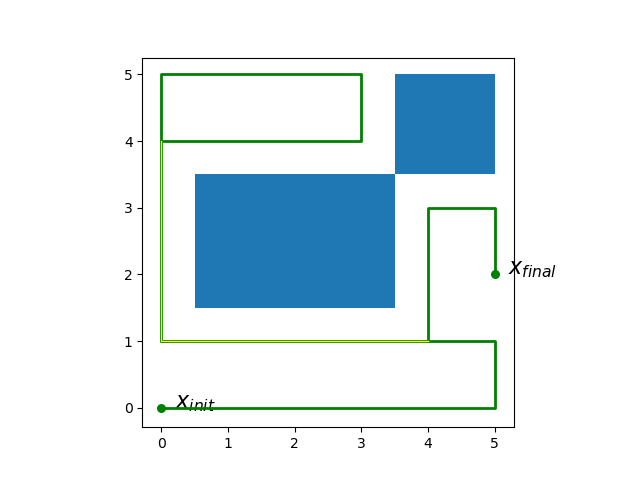
\includegraphics[width=\linewidth]{deliverables/DLS_2_obs.png}
      \caption{depth-limited Search 2 obstacle case }
    \end{minipage}
        \begin{minipage}{.33\textwidth}
      \centering
      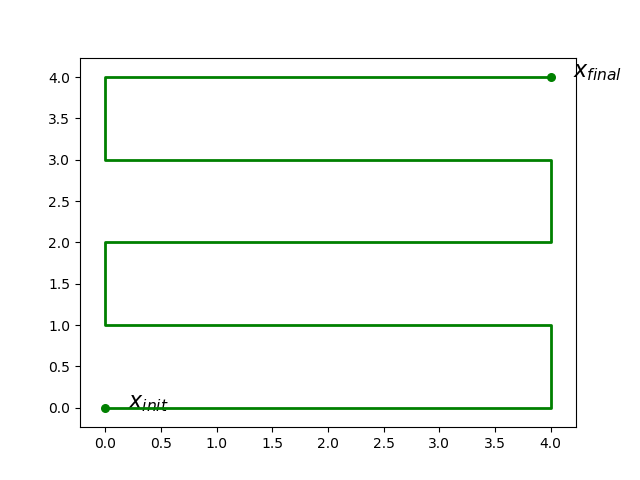
\includegraphics[width=\linewidth]{deliverables/LAS_no_obs.png}
      \caption{Local-approximation Search no obstacle case }
    \end{minipage}%
            \begin{minipage}{.33\textwidth}
      \centering
      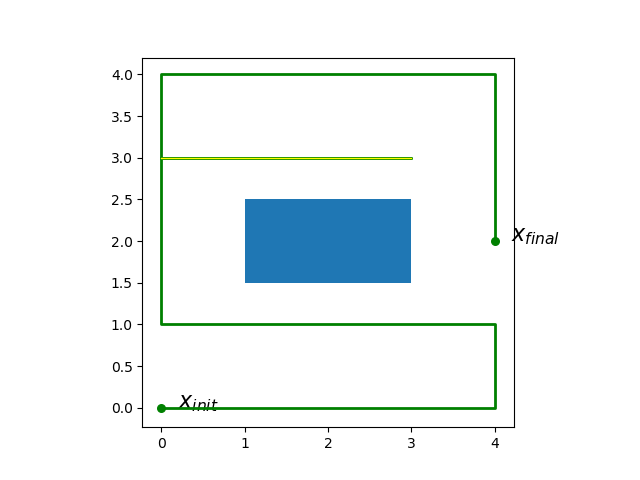
\includegraphics[width=\linewidth]{deliverables/LAS_1_obs.png}
      \caption{Local-approximation Search 1 obstacle case }
    \end{minipage}%
            \begin{minipage}{.33\textwidth}
      \centering
      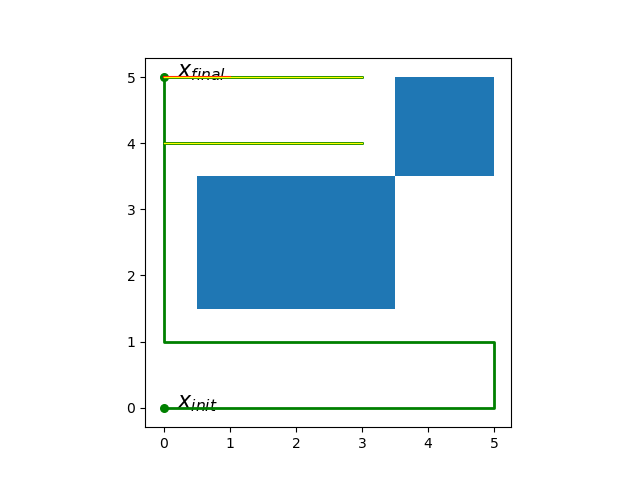
\includegraphics[width=\linewidth]{deliverables/LAS_2_obs.png}
      \caption{Local-approximation Search 2 obstacle case }
    \end{minipage}
    \caption{The algorithm performance of A*, depth-limited Search and Local-approximation Search.}
    \label{fig:algovsA*}
    \end{figure}
            
\begin{table}[!htbp]
\centering
\caption{Comparison of performance.}
\begin{tabular}{*4c}
\toprule
Map &  Algorithm & Turn number & Total Distance\\
\midrule
\multirow{ 3}{*}{No obstacle}  & A*   &   8  & 25 \\
   &  Depth-limited Search & 8   & 27  \\
   &  Local-approximation Search & 8   & 25  \\
   \midrule
\multirow{ 3}{*}{1 obstacle}   &  A*  &  7   & 26 \\
  & Depth-limited Search & 9   & 26\\
    &  Local-approximation Search & 8   & 25  \\
    \midrule
    \multirow{ 3}{*}{2 obstacle}   &  A*  &  8   & 26 \\
  & Depth-limited Search & 11   & 34\\
    &  Local-approximation Search &  nan & nan  \\
\bottomrule
\label{comparison table}
\end{tabular}
\end{table}
            
        
    \end{normalsize}
  
  \newpage
    \begin{thebibliography}{00}
        \bibitem{b1}A. Ntawumenyikizaba, Hoang Huu Viet and TaeChoong Chung, "An online complete coverage algorithm for cleaning robots based on boustrophedon motions and A* search," 2012 8th International Conference on Information Science and Digital Content Technology (ICIDT2012), Jeju, 2012, pp. 401-405.
        \bibitem{b2}Peng Zhou and Zhong-min Wang and Zhen-nan Li and Yang Li, "Complete Coverage Path Planning of Mobile Robot Based on Dynamic Programming Algorithm", 2nd International Conference on Electronic \& Mechanical Engineering and Information Technology, 2012
        \bibitem{b3}Galceran, Enric, and Marc Carreras. "A survey on coverage path planning for robotics." Robotics and Autonomous systems 61.12 (2013): 1258-1276.
        \bibitem{b4}Luis Piardi, José Lima, Ana I. Pereira, and Paulo Costa. "Coverage path planning optimization based
        on Q-learning algorithm"AIP Conference Proceedings 2116, 220002 (2019)
        
    \end{thebibliography}
    
\end{document}
